\documentclass{article}
\usepackage[letterpaper]{geometry}
\geometry{verbose,tmargin=1in,bmargin=1in,lmargin=1in,rmargin=1in}

\usepackage[utf8]{inputenc}
\usepackage{amsmath}
\usepackage{listings}
\usepackage{graphicx}
\usepackage{enumitem}

\title{CIS 419/519: Homework 2}
\author{Jiatong Sun}
\date{}

\begin{document}
    \maketitle
	Although the solutions are entirely my own, I consulted with the following people and sources while working on this homework: $Junfan Pan$ \\
    $https://machinelearningmastery.com/understand-the-dynamics-of-learning-rate-on-deep-learning-neural-networks/$\\
    $https://en.wikipedia.org/wiki/Learning_rate$\\
    $https://machinelearningmastery.com/how-to-tune-algorithm-parameters-with-scikit-learn/$.
    
    \section{Gradient Descent}
        \begin{enumerate}[label=\alph*.]
            \item % a
            The implication of the learning rate $\alpha_{k}$ is to control how big a step should be taken in the gradient descent direction towards the minimum, where a too small $\alpha_{k}$ may result in a long training time and a too large $\alpha_{k}$ may lead to an overshooting training process.
            
            
            \item % b
            The implications of setting $\alpha_{k}$ as a function of k is to select an adaptive learning rate based on the training process, since the best step to take can vary as the the training goes gradually towards the minimum and a preset constant $\alpha_{k}$ may not work well in the whole process.
        \end{enumerate}
        
       \section{Linear Regression [CIS 519 ONLY]}
       
       \section{Polynomial Regression}
        
        \begin{figure}[h]
			\centering
			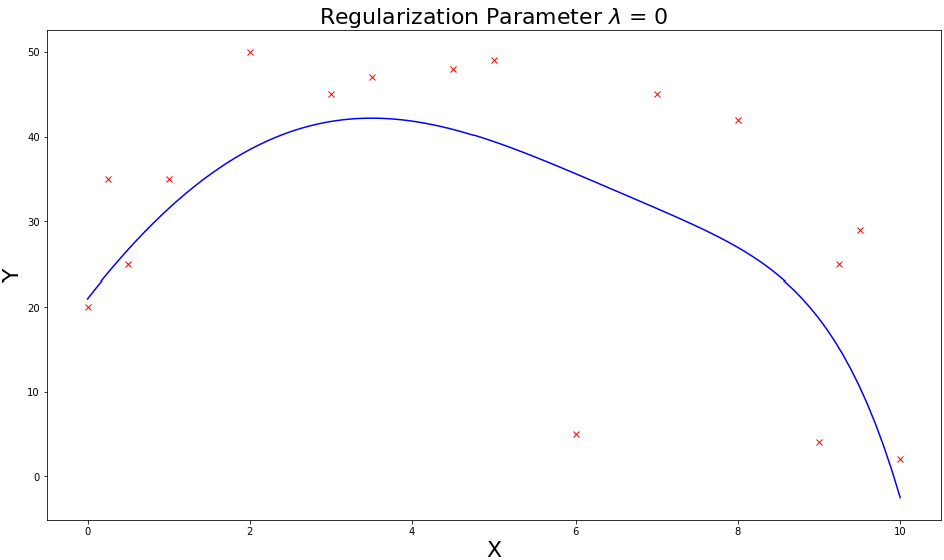
\includegraphics[width=0.8\textwidth]
            {fig_1.png}
            \caption{$\lambda = 0$}
            \label{fig:1}
		\end{figure}    
		
		\begin{figure}[h]
			\centering
			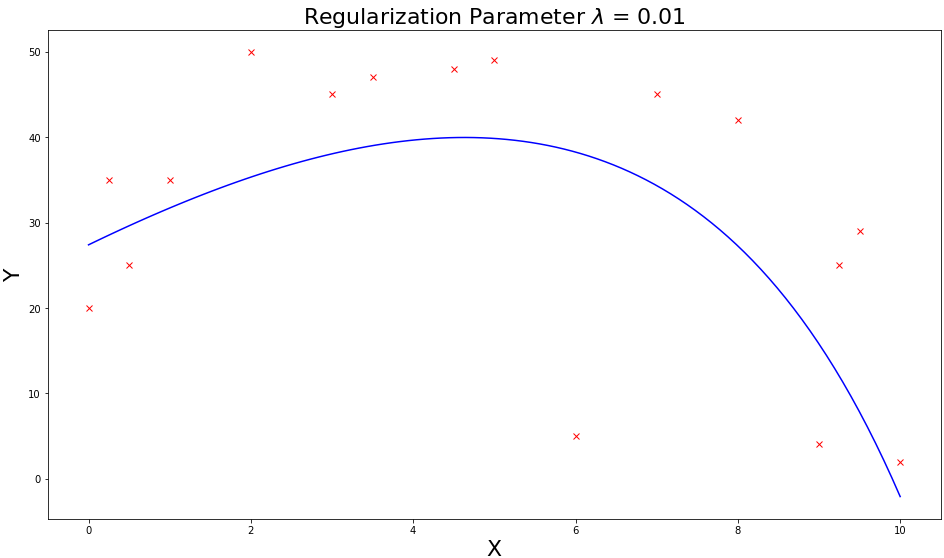
\includegraphics[width=0.8\textwidth]
            {fig_2.png}
            \caption{$\lambda = 0.01$}
            \label{fig:2}
		\end{figure}    
        
\end{document}